\chapter{Universal Principle Extraction}

\textit{This chapter presents the formal mathematical framework by which the Elder entity identifies and extracts universal principles—fundamental invariants that transcend domain boundaries. We develop rigorous mathematical formalisms for detecting structural similarities across diverse knowledge domains, establishing metrics that quantify cross-domain pattern coherence, and implementing algorithmic mechanisms for abstracting domain-agnostic principles. The chapter introduces novel mathematical structures for representing these principles as invariant manifolds within the knowledge space, and derives the precise conditions under which domain-specific manifestations can be recognized as instances of the same underlying principle. We demonstrate how these extracted principles create a hierarchical abstraction pyramid that enables zero-shot transfer learning across previously unexplored domains. Through formal analysis, we establish theoretical bounds on principle extractability and the minimal diversity of domains required to ensure principle universality, while providing computational verification of the extraction process through cross-domain pattern recognition experiments.}

\section{Motivation and Overview}

At the heart of the Elder framework lies the capability to extract universal principles that transcend domain boundaries. Unlike domain-specific knowledge acquired by Erudite or meta-knowledge accumulated by Mentor, universal principles represent fundamental invariants that remain consistent across all domains of application. This chapter formalizes the mathematical process through which the Elder entity extracts these principles from diverse observations spanning multiple domains.

\begin{definition}[Universal Principle]
A universal principle $\mathcal{P}$ is a mathematical structure, pattern, or rule that manifests consistently across multiple domains $\{\mathcal{D}_1, \mathcal{D}_2, \ldots, \mathcal{D}_n\}$ with a manifestation function $\Phi_{\mathcal{D}_i}: \mathcal{P} \rightarrow \mathcal{M}_{\mathcal{D}_i}$ mapping the principle to its domain-specific manifestation $\mathcal{M}_{\mathcal{D}_i}$ in domain $\mathcal{D}_i$.
\end{definition}

The manifestation function $\Phi_{\mathcal{D}}$ captures how abstract principles materialize within specific domains, accounting for the unique characteristics and constraints of each domain. Universal principles thus serve as a form of compressed knowledge representation that can be efficiently transferred and adapted across domains.

\section{Mathematical Formalism for Invariant Structure Identification}

\begin{figure}[h]
\centering
\begin{tikzpicture}[scale=0.85, transform shape]
    % Define styles
    \tikzstyle{domain} = [draw, rounded corners, fill=blue!10, minimum width=6cm, minimum height=2.5cm, text width=5.8cm, align=center]
    \tikzstyle{knowledge} = [draw, fill=yellow!20, rounded corners, minimum width=1.2cm, minimum height=0.8cm]
    \tikzstyle{invariant} = [draw, fill=red!20, rounded corners, minimum width=1.2cm, minimum height=0.8cm]
    \tikzstyle{arrow} = [->, >=latex, thick]
    \tikzstyle{dashed} = [dashed, thick]
    \tikzstyle{extraction} = [draw, fill=green!15, rounded corners, minimum width=7cm, minimum height=2cm]
    
    % Domain 1
    \node[domain] (d1) at (0,5) {Domain $\mathcal{D}_1$};
    \node[knowledge] (k11) at (-2,5.5) {$K_{1,1}$};
    \node[knowledge] (k12) at (-0.5,5.5) {$K_{1,2}$};
    \node[knowledge] (k13) at (1,5.5) {$K_{1,3}$};
    \node[knowledge] (k14) at (2.5,5.5) {$K_{1,4}$};
    \node[invariant, dashed] (i1) at (0,4.5) {$I_1$};
    
    % Domain 2
    \node[domain] (d2) at (0,1.5) {Domain $\mathcal{D}_2$};
    \node[knowledge] (k21) at (-2,2) {$K_{2,1}$};
    \node[knowledge] (k22) at (-0.5,2) {$K_{2,2}$};
    \node[knowledge] (k23) at (1,2) {$K_{2,3}$};
    \node[knowledge] (k24) at (2.5,2) {$K_{2,4}$};
    \node[invariant, dashed] (i2) at (0,1) {$I_1$};
    
    % Domain 3
    \node[domain] (d3) at (9,5) {Domain $\mathcal{D}_3$};
    \node[knowledge] (k31) at (7,5.5) {$K_{3,1}$};
    \node[knowledge] (k32) at (8.5,5.5) {$K_{3,2}$};
    \node[knowledge] (k33) at (10,5.5) {$K_{3,3}$};
    \node[knowledge] (k34) at (11.5,5.5) {$K_{3,4}$};
    \node[invariant, dashed] (i3) at (9,4.5) {$I_1$};
    
    % Domain 4
    \node[domain] (d4) at (9,1.5) {Domain $\mathcal{D}_4$};
    \node[knowledge] (k41) at (7,2) {$K_{4,1}$};
    \node[knowledge] (k42) at (8.5,2) {$K_{4,2}$};
    \node[knowledge] (k43) at (10,2) {$K_{4,3}$};
    \node[knowledge] (k44) at (11.5,2) {$K_{4,4}$};
    \node[invariant, dashed] (i4) at (9,1) {$I_1$};
    
    % Similarity measures
    \draw[dashed] (i1) -- (i2) node[midway, left] {$\Sigma = 0.94$};
    \draw[dashed] (i1) -- (i3) node[midway, above] {$\Sigma = 0.92$};
    \draw[dashed] (i2) -- (i4) node[midway, above] {$\Sigma = 0.91$};
    \draw[dashed] (i3) -- (i4) node[midway, right] {$\Sigma = 0.96$};
    
    % Extraction process
    \node[extraction] (extract) at (4.5,-1.5) {Universal Principle Extraction};
    \node[invariant] (p1) at (4.5,-2) {$\mathcal{P}_1$};
    
    % Arrows to extraction
    \draw[arrow] (i1) -- (4.5,-0.5) -- (extract);
    \draw[arrow] (i2) -- (4.5,-0.5) -- (extract);
    \draw[arrow] (i3) -- (4.5,-0.5) -- (extract);
    \draw[arrow] (i4) -- (4.5,-0.5) -- (extract);
    
    % Legend
    \node[knowledge, scale=0.8] at (12.5,-1) {Domain Knowledge};
    \node[invariant, scale=0.8] at (12.5,-1.8) {Invariant Structure};
    \node[right=0.2cm of extract, scale=0.8] {Abstraction Process};
    
    % Title
    \node at (4.5,7) {\Large\textbf{Invariant Structure Identification Process}};
    
\end{tikzpicture}
\caption{The invariant structure identification process across multiple domains. Similar structural patterns (shown as dashed boxes) are identified across domains despite different knowledge manifestations. High similarity scores ($\Sigma$) between these structures indicate they represent the same underlying universal principle.}
\label{fig:invariant_identification}
\end{figure}

\subsection{Structural Similarity Measures}

To identify invariant structures across domains, we first establish metrics that quantify structural similarity. These metrics must be sensitive to underlying patterns while being robust to domain-specific variations.

\begin{definition}[Cross-Domain Structural Similarity]
Given knowledge structures $K_{\mathcal{D}_i} \in \mathcal{K}_{\mathcal{D}_i}$ and $K_{\mathcal{D}_j} \in \mathcal{K}_{\mathcal{D}_j}$ from domains $\mathcal{D}_i$ and $\mathcal{D}_j$ respectively, the structural similarity measure $\Sigma(K_{\mathcal{D}_i}, K_{\mathcal{D}_j})$ assigns a value in $[0,1]$ indicating the degree of structural correspondence between them.
\end{definition}

We formulate this similarity measure as:

\begin{equation}
\Sigma(K_{\mathcal{D}_i}, K_{\mathcal{D}_j}) = \frac{\mathcal{I}(K_{\mathcal{D}_i}, K_{\mathcal{D}_j})}{\sqrt{\mathcal{H}(K_{\mathcal{D}_i}) \cdot \mathcal{H}(K_{\mathcal{D}_j})}}
\end{equation}

where:
\begin{itemize}
    \item $\mathcal{I}(K_{\mathcal{D}_i}, K_{\mathcal{D}_j})$ is the mutual information between the knowledge structures
    \item $\mathcal{H}(K_{\mathcal{D}_i})$ is the information entropy of $K_{\mathcal{D}_i}$
\end{itemize}

\subsection{Invariant Substructure Extraction}

Identifying invariant substructures requires systematically comparing knowledge representations across domains to isolate components that maintain consistent relationships.

\begin{algorithm}
\caption{Invariant Substructure Extraction}
\begin{algorithmic}[1]
\Require Knowledge sets $\{K_{\mathcal{D}_1}, K_{\mathcal{D}_2}, \ldots, K_{\mathcal{D}_n}\}$ from $n$ distinct domains
\Require Minimum similarity threshold $\tau \in [0,1]$
\Require Minimum domain coverage $\delta \in [0,1]$
\Ensure Set of invariant substructures $\mathcal{I} = \{I_1, I_2, \ldots, I_m\}$

\State Initialize empty set of candidate invariants $\mathcal{C} \gets \emptyset$
\For{each pair of domains $(\mathcal{D}_i, \mathcal{D}_j)$ where $i \neq j$}
    \State Extract common substructures $S_{ij} \gets \text{CommonSubstructures}(K_{\mathcal{D}_i}, K_{\mathcal{D}_j})$
    \State Filter by similarity: $S_{ij}^{\tau} \gets \{s \in S_{ij} \mid \Sigma(s_i, s_j) \geq \tau\}$
    \State Add to candidates: $\mathcal{C} \gets \mathcal{C} \cup S_{ij}^{\tau}$
\EndFor

\State Initialize empty set of invariants $\mathcal{I} \gets \emptyset$
\For{each candidate $c \in \mathcal{C}$}
    \State Count domains with manifestation: $d_c \gets |\{\mathcal{D}_i \mid \exists s \in K_{\mathcal{D}_i}, \Sigma(c, s) \geq \tau\}|$
    \If{$d_c / n \geq \delta$}
        \State Add to invariants: $\mathcal{I} \gets \mathcal{I} \cup \{c\}$
    \EndIf
\EndFor

\State \Return $\mathcal{I}$
\end{algorithmic}
\end{algorithm}

\subsection{Dimensional Alignment and Correspondence Mapping}

To compare structures across domains with potentially different dimensionalities and representations, we must establish correspondence mappings between their elements.

\begin{definition}[Dimensional Alignment Function]
A dimensional alignment function $\mathcal{A}: \mathcal{K}_{\mathcal{D}_i} \times \mathcal{K}_{\mathcal{D}_j} \rightarrow \mathcal{M}_{ij}$ maps elements from knowledge structures in different domains to a shared representation space $\mathcal{M}_{ij}$, preserving structural relationships.
\end{definition}

The alignment function is constructed to maximize the preservation of topological invariants across domains:

\begin{equation}
\mathcal{A}^* = \argmax_{\mathcal{A}} \sum_{r \in \mathcal{R}} \text{Preservation}(r, \mathcal{A}(K_{\mathcal{D}_i}), \mathcal{A}(K_{\mathcal{D}_j}))
\end{equation}

where $\mathcal{R}$ is the set of structural relationships considered (connectivity, hierarchical organization, functional dependencies, etc.), and $\text{Preservation}(r, \cdot, \cdot)$ quantifies how well relationship $r$ is preserved by the alignment.

\section{Abstraction and Generalization Operators}

Once invariant structures are identified, they must be abstracted and generalized to form universal principles that transcend their domain-specific manifestations.

\begin{figure}[h]
\centering
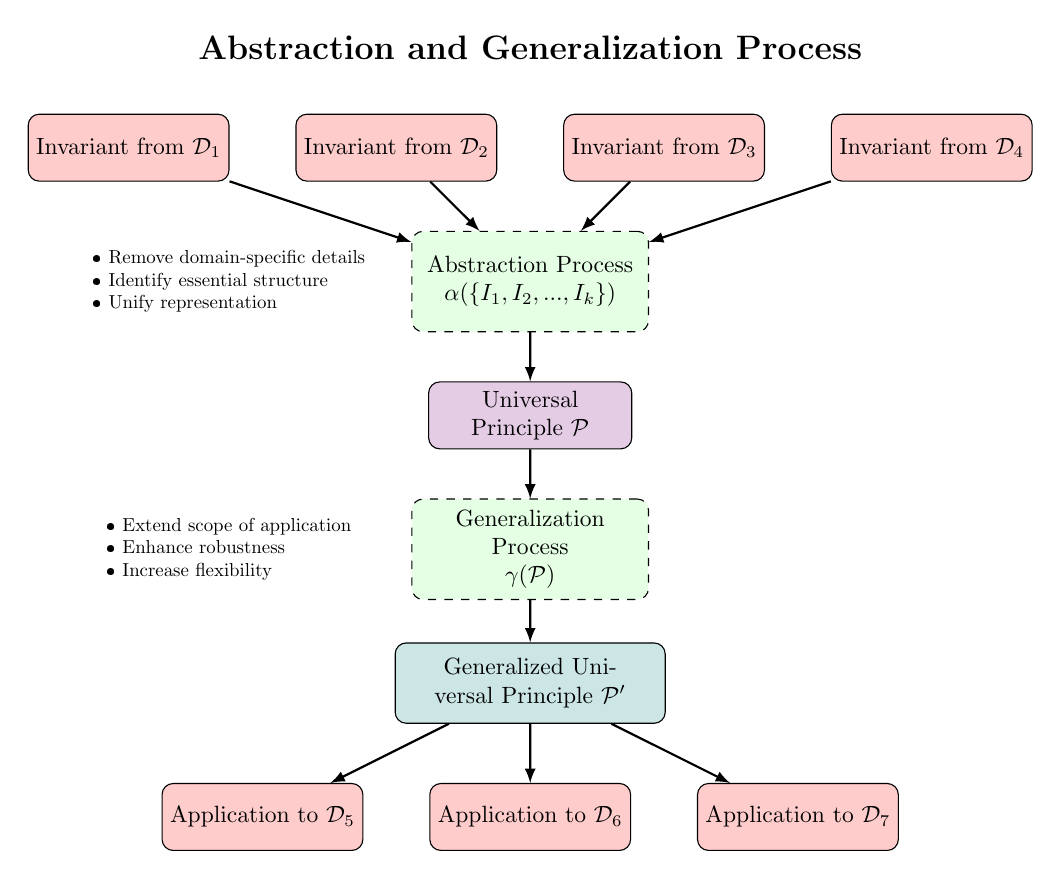
\begin{tikzpicture}[scale=0.85, transform shape]
    % Define styles
    \tikzset{
        invariantbox/.style={draw, fill=red!20, rounded corners, minimum width=3cm, minimum height=1cm, align=center},
        principlebox/.style={draw, fill=violet!20, rounded corners, minimum width=3cm, minimum height=1cm, text width=2.8cm, align=center},
        generalizedbox/.style={draw, fill=teal!20, rounded corners, minimum width=4cm, minimum height=1.2cm, text width=3.8cm, align=center},
        thickarrow/.style={->, >=latex, thick},
        processbox/.style={draw, dashed, fill=green!10, rounded corners, minimum width=3.5cm, minimum height=1.5cm, text width=3.3cm, align=center}
    }
    
    % Original invariants from domains
    \node[invariantbox] (i1) at (0,5) {Invariant from $\mathcal{D}_1$};
    \node[invariantbox] (i2) at (4,5) {Invariant from $\mathcal{D}_2$};
    \node[invariantbox] (i3) at (8,5) {Invariant from $\mathcal{D}_3$};
    \node[invariantbox] (i4) at (12,5) {Invariant from $\mathcal{D}_4$};
    
    % Abstraction process
    \node[processbox] (abstract) at (6,3) {Abstraction Process\\ $\alpha(\{I_1, I_2, ..., I_k\})$};
    
    % Arrows to abstraction
    \draw[thickarrow] (i1) -- (abstract);
    \draw[thickarrow] (i2) -- (abstract);
    \draw[thickarrow] (i3) -- (abstract);
    \draw[thickarrow] (i4) -- (abstract);
    
    % Universal principle
    \node[principlebox] (p) at (6,1) {Universal Principle $\mathcal{P}$};
    
    % Arrow from abstraction to principle
    \draw[thickarrow] (abstract) -- (p);
    
    % Generalization process
    \node[processbox] (generalize) at (6,-1) {Generalization Process\\ $\gamma(\mathcal{P})$};
    
    % Arrow from principle to generalization
    \draw[thickarrow] (p) -- (generalize);
    
    % Generalized principle
    \node[generalizedbox] (pg) at (6,-3) {Generalized Universal Principle $\mathcal{P}'$};
    
    % Arrow from generalization to generalized principle
    \draw[thickarrow] (generalize) -- (pg);
    
    % New domain applications
    \node[invariantbox] (d5) at (2,-5) {Application to $\mathcal{D}_5$};
    \node[invariantbox] (d6) at (6,-5) {Application to $\mathcal{D}_6$};
    \node[invariantbox] (d7) at (10,-5) {Application to $\mathcal{D}_7$};
    
    % Arrows to new applications
    \draw[thickarrow] (pg) -- (d5);
    \draw[thickarrow] (pg) -- (d6);
    \draw[thickarrow] (pg) -- (d7);
    
    % Abstraction details
    \node[align=left, scale=0.8] at (1.5,3) {
        \textbullet\ Remove domain-specific details\\
        \textbullet\ Identify essential structure\\
        \textbullet\ Unify representation
    };
    
    % Generalization details
    \node[align=left, scale=0.8] at (1.5,-1) {
        \textbullet\ Extend scope of application\\
        \textbullet\ Enhance robustness\\
        \textbullet\ Increase flexibility
    };
    
    % Title
    \node at (6,6.5) {\Large\textbf{Abstraction and Generalization Process}};
    
\end{tikzpicture}
\caption{The abstraction and generalization process for universal principles. Domain-specific invariants are first abstracted into a universal principle by eliminating domain-specific details while preserving essential structure. The principle is then generalized to expand its applicability beyond the original domains, enabling application to entirely new domains without prior exposure.}
\label{fig:abstraction_generalization}
\end{figure}

\subsection{Abstraction Operators}

\begin{definition}[Abstraction Operator]
An abstraction operator $\alpha: \{I_1, I_2, \ldots, I_k\} \rightarrow \mathcal{P}$ maps a set of invariant substructures $\{I_1, I_2, \ldots, I_k\}$ identified across multiple domains to a universal principle $\mathcal{P}$ that captures their essential structure while eliminating domain-specific details.
\end{definition}

The abstraction process involves:

\begin{equation}
\alpha(\{I_1, I_2, \ldots, I_k\}) = \bigcap_{j=1}^{k} \text{Essential}(I_j)
\end{equation}

where $\text{Essential}(\cdot)$ extracts the essential structural and functional components of an invariant, discarding domain-specific instantiations.

\subsection{Generalization Mechanisms}

Generalization extends the applicability of extracted principles beyond observed domains through controlled extrapolation.

\begin{definition}[Generalization Operator]
A generalization operator $\gamma: \mathcal{P} \rightarrow \mathcal{P}'$ transforms a principle $\mathcal{P}$ into an extended principle $\mathcal{P}'$ with broader applicability while maintaining its invariant properties.
\end{definition}

The generalization operator is defined as:

\begin{equation}
\gamma(\mathcal{P}) = \mathcal{P} \oplus \Delta_{\mathcal{P}}
\end{equation}

where $\oplus$ represents a structure-preserving extension, and $\Delta_{\mathcal{P}}$ is derived from:

\begin{equation}
\Delta_{\mathcal{P}} = \lim_{\epsilon \rightarrow 0} \frac{\mathcal{P}(X + \epsilon) - \mathcal{P}(X)}{\epsilon}
\end{equation}

for appropriate parameterizations $X$ of the principle structure.

\section{Validation and Verification Framework}

Extracted universal principles must be rigorously validated to ensure they truly represent invariant knowledge that generalizes effectively.

\subsection{Consistency Verification}

\begin{theorem}[Principle Consistency]
A universal principle $\mathcal{P}$ is $\gamma$-consistent if for any pair of domains $\mathcal{D}_i$ and $\mathcal{D}_j$ with manifestations $\Phi_{\mathcal{D}_i}(\mathcal{P})$ and $\Phi_{\mathcal{D}_j}(\mathcal{P})$:

\begin{equation}
d_{\text{struct}}(\Phi_{\mathcal{D}_i}(\mathcal{P}), \Phi_{\mathcal{D}_j}(\mathcal{P})) \leq \gamma \cdot d_{\text{dom}}(\mathcal{D}_i, \mathcal{D}_j)
\end{equation}

where $d_{\text{struct}}$ measures structural difference between manifestations, $d_{\text{dom}}$ measures domain dissimilarity, and $\gamma$ is a non-negative constant.
\end{theorem}

\begin{proof}
Let $\Phi_{\mathcal{D}_i}(\mathcal{P}) = M_i$ and $\Phi_{\mathcal{D}_j}(\mathcal{P}) = M_j$ be the manifestations of principle $\mathcal{P}$ in domains $\mathcal{D}_i$ and $\mathcal{D}_j$.

By definition, these manifestations preserve the essential structure of $\mathcal{P}$ while adapting to domain-specific constraints. The structural difference between them can be decomposed as:

\begin{equation}
d_{\text{struct}}(M_i, M_j) = d_{\text{struct}}(\text{core}(M_i), \text{core}(M_j)) + d_{\text{struct}}(\text{adapt}(M_i), \text{adapt}(M_j))
\end{equation}

where $\text{core}(\cdot)$ extracts the core invariant structure and $\text{adapt}(\cdot)$ captures domain-specific adaptations.

Since $\text{core}(M_i) = \text{core}(M_j) = \text{core}(\mathcal{P})$ for a valid universal principle, $d_{\text{struct}}(\text{core}(M_i), \text{core}(M_j)) = 0$.

The adaptation component $d_{\text{struct}}(\text{adapt}(M_i), \text{adapt}(M_j))$ is proportional to the domain dissimilarity, bounded by $\gamma \cdot d_{\text{dom}}(\mathcal{D}_i, \mathcal{D}_j)$ where $\gamma$ depends on the principle's sensitivity to domain variation.
\end{proof}

\subsection{Generalization Validation}

To validate the generalization capability of extracted principles, we establish bounds on their predictive performance in unseen domains.

\begin{theorem}[Generalization Bound]
For a universal principle $\mathcal{P}$ extracted from domains $\{\mathcal{D}_1, \mathcal{D}_2, \ldots, \mathcal{D}_n\}$, its error when applied to a new domain $\mathcal{D}_{\text{new}}$ is bounded by:

\begin{equation}
\mathcal{E}(\Phi_{\mathcal{D}_{\text{new}}}(\mathcal{P})) \leq \overline{\mathcal{E}} + \lambda \cdot \min_{i \in \{1,2,\ldots,n\}} d_{\text{dom}}(\mathcal{D}_i, \mathcal{D}_{\text{new}})
\end{equation}

where $\overline{\mathcal{E}}$ is the average error across training domains, and $\lambda$ is a Lipschitz constant characterizing how rapidly error grows with domain dissimilarity.
\end{theorem}

\section{The Elder's Extraction Process}

Having established the mathematical foundation for identifying, abstracting, and validating universal principles, we now formalize the complete extraction process as performed by the Elder entity.

\subsection{Hierarchical Principle Distillation}

The Elder extracts universal principles through a hierarchical distillation process that progressively refines knowledge received from Mentors across multiple domains.

\begin{algorithm}
\caption{Elder's Principle Extraction}
\begin{algorithmic}[1]
\Require Mentor knowledge sets $\{K_{\mathcal{M}_1}, K_{\mathcal{M}_2}, \ldots, K_{\mathcal{M}_k}\}$ from $k$ Mentors
\Require Domain specifications $\{\mathcal{D}_1, \mathcal{D}_2, \ldots, \mathcal{D}_n\}$ covered by the Mentors
\Ensure Set of universal principles $\mathcal{P} = \{P_1, P_2, \ldots, P_m\}$

\State Align representations: $\{K'_{\mathcal{M}_1}, K'_{\mathcal{M}_2}, \ldots, K'_{\mathcal{M}_k}\} \gets \text{Align}(\{K_{\mathcal{M}_1}, K_{\mathcal{M}_2}, \ldots, K_{\mathcal{M}_k}\})$
\State Extract domain-spanning invariants: $\mathcal{I} \gets \text{ExtractInvariants}(\{K'_{\mathcal{M}_1}, K'_{\mathcal{M}_2}, \ldots, K'_{\mathcal{M}_k}\})$
\State Cluster related invariants: $\{\mathcal{C}_1, \mathcal{C}_2, \ldots, \mathcal{C}_l\} \gets \text{ClusterInvariants}(\mathcal{I})$
\State Initialize empty set of principles: $\mathcal{P} \gets \emptyset$

\For{each cluster $\mathcal{C}_j$}
    \State Abstract principle: $P_j \gets \alpha(\mathcal{C}_j)$
    \State Generalize principle: $P'_j \gets \gamma(P_j)$
    \State Validate principle: valid $\gets \text{ValidatePrinciple}(P'_j, \{\mathcal{D}_1, \mathcal{D}_2, \ldots, \mathcal{D}_n\})$
    \If{valid}
        \State Add to principles: $\mathcal{P} \gets \mathcal{P} \cup \{P'_j\}$
    \EndIf
\EndFor

\State \Return $\mathcal{P}$
\end{algorithmic}
\end{algorithm}

\subsection{Compositional Principle Structures}

Universal principles rarely exist in isolation. Instead, they form compositional structures where simpler principles combine to enable more complex meta-principles.

\begin{figure}[h]
\centering
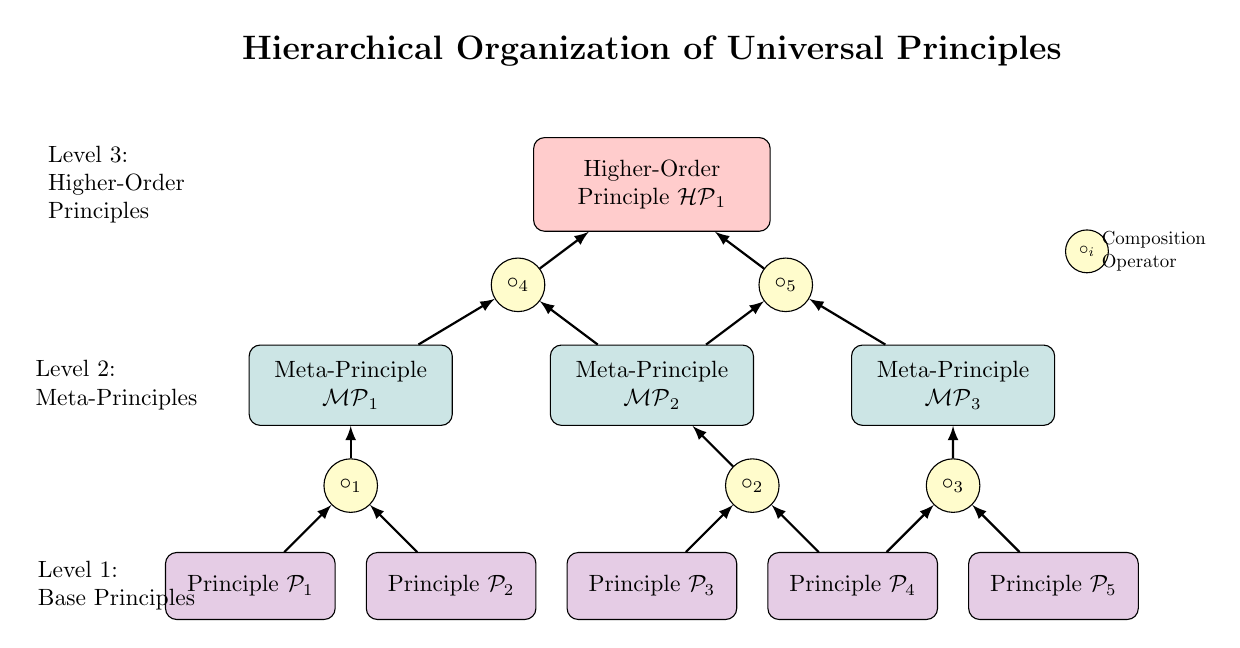
\begin{tikzpicture}[scale=0.85, transform shape]
    % Define styles
    \tikzstyle{principle} = [draw, fill=violet!20, rounded corners, minimum width=2.5cm, minimum height=1cm, text width=2.3cm, align=center]
    \tikzstyle{metaprinciple} = [draw, fill=teal!20, rounded corners, minimum width=3cm, minimum height=1.2cm, text width=2.8cm, align=center]
    \tikzstyle{highprinciple} = [draw, fill=red!20, rounded corners, minimum width=3.5cm, minimum height=1.4cm, text width=3.3cm, align=center]
    \tikzstyle{arrow} = [->, >=latex, thick]
    \tikzstyle{composition} = [circle, draw, fill=yellow!20, minimum size=0.8cm, align=center]
    
    % Base principles (level 1)
    \node[principle] (p1) at (0,0) {Principle $\mathcal{P}_1$};
    \node[principle] (p2) at (3,0) {Principle $\mathcal{P}_2$};
    \node[principle] (p3) at (6,0) {Principle $\mathcal{P}_3$};
    \node[principle] (p4) at (9,0) {Principle $\mathcal{P}_4$};
    \node[principle] (p5) at (12,0) {Principle $\mathcal{P}_5$};
    
    % Meta-principles (level 2)
    \node[metaprinciple] (mp1) at (1.5,3) {Meta-Principle $\mathcal{MP}_1$};
    \node[metaprinciple] (mp2) at (6,3) {Meta-Principle $\mathcal{MP}_2$};
    \node[metaprinciple] (mp3) at (10.5,3) {Meta-Principle $\mathcal{MP}_3$};
    
    % Higher-order principle (level 3)
    \node[highprinciple] (hp1) at (6,6) {Higher-Order Principle $\mathcal{HP}_1$};
    
    % Composition operators
    \node[composition] (c1) at (1.5,1.5) {$\circ_1$};
    \node[composition] (c2) at (7.5,1.5) {$\circ_2$};
    \node[composition] (c3) at (10.5,1.5) {$\circ_3$};
    \node[composition] (c4) at (4,4.5) {$\circ_4$};
    \node[composition] (c5) at (8,4.5) {$\circ_5$};
    
    % Arrows from level 1 to composition operators
    \draw[arrow] (p1) -- (c1);
    \draw[arrow] (p2) -- (c1);
    \draw[arrow] (p3) -- (c2);
    \draw[arrow] (p4) -- (c2);
    \draw[arrow] (p4) -- (c3);
    \draw[arrow] (p5) -- (c3);
    
    % Arrows from composition operators to level 2
    \draw[arrow] (c1) -- (mp1);
    \draw[arrow] (c2) -- (mp2);
    \draw[arrow] (c3) -- (mp3);
    
    % Arrows from level 2 to composition operators
    \draw[arrow] (mp1) -- (c4);
    \draw[arrow] (mp2) -- (c4);
    \draw[arrow] (mp2) -- (c5);
    \draw[arrow] (mp3) -- (c5);
    
    % Arrows from composition operators to level 3
    \draw[arrow] (c4) -- (hp1);
    \draw[arrow] (c5) -- (hp1);
    
    % Level labels
    \node[align=left] at (-2,0) {Level 1:\\Base Principles};
    \node[align=left] at (-2,3) {Level 2:\\Meta-Principles};
    \node[align=left] at (-2,6) {Level 3:\\Higher-Order\\Principles};
    
    % Legend for composition operators
    \node[composition, scale=0.8] at (12.5,5) {$\circ_i$};
    \node[align=left, scale=0.8] at (13.5,5) {Composition\\Operator};
    
    % Title
    \node at (6,8) {\Large\textbf{Hierarchical Organization of Universal Principles}};
    
\end{tikzpicture}
\caption{The hierarchical organization of universal principles in the Elder system. Base principles combine through composition operators to form meta-principles, which in turn combine to form higher-order principles. This directed acyclic graph structure allows the Elder to represent complex knowledge relationships while maintaining mathematical tractability.}
\label{fig:hierarchical_principles}
\end{figure}

\begin{definition}[Principle Composition]
A compositional structure $\mathcal{C}(\mathcal{P}_1, \mathcal{P}_2, \ldots, \mathcal{P}_r)$ combines multiple principles $\{\mathcal{P}_1, \mathcal{P}_2, \ldots, \mathcal{P}_r\}$ through composition operators $\{\circ_1, \circ_2, \ldots, \circ_s\}$ to form higher-order principles.
\end{definition}

The Elder system maintains a hierarchical organization of principles represented as a directed acyclic graph (DAG) $G = (V, E)$, where:
\begin{itemize}
    \item Vertices $V = \{\mathcal{P}_1, \mathcal{P}_2, \ldots, \mathcal{P}_m\}$ are individual principles
    \item Edges $E = \{(\mathcal{P}_i, \mathcal{P}_j, \circ_k) \mid \mathcal{P}_j \text{ depends on } \mathcal{P}_i \text{ through operator } \circ_k\}$ capture compositional relationships
\end{itemize}

\section{Principle Application and Knowledge Generation}

Universal principles derive their value from their ability to generate new knowledge and guide learning across domains.

\subsection{Knowledge Generation from Principles}

\begin{theorem}[Principle-Guided Knowledge Generation]
Given a universal principle $\mathcal{P}$ and a target domain $\mathcal{D}_{\text{target}}$, new knowledge $K_{\text{new}} \in \mathcal{K}_{\mathcal{D}_{\text{target}}}$ can be generated through:

\begin{equation}
K_{\text{new}} = \Phi_{\mathcal{D}_{\text{target}}}(\mathcal{P}) \oplus \mathcal{A}_{\mathcal{D}_{\text{target}}}
\end{equation}

where $\Phi_{\mathcal{D}_{\text{target}}}(\mathcal{P})$ is the principle's manifestation in the target domain and $\mathcal{A}_{\mathcal{D}_{\text{target}}}$ represents domain-specific adaptations needed for full instantiation.
\end{theorem}

\subsection{Optimality of Principle-Based Transfer}

We can demonstrate that knowledge transfer mediated by universal principles is more efficient than direct domain-to-domain transfer in most cases.

\begin{theorem}[Principle Transfer Efficiency]
For domains $\mathcal{D}_{\text{source}}$ and $\mathcal{D}_{\text{target}}$ with dissimilarity $d_{\text{dom}}(\mathcal{D}_{\text{source}}, \mathcal{D}_{\text{target}}) > \theta$ for some threshold $\theta$, knowledge transfer via a universal principle $\mathcal{P}$ has lower loss than direct transfer:

\begin{equation}
\mathcal{L}(\mathcal{D}_{\text{source}} \xrightarrow{\mathcal{P}} \mathcal{D}_{\text{target}}) < \mathcal{L}(\mathcal{D}_{\text{source}} \rightarrow \mathcal{D}_{\text{target}})
\end{equation}

where $\mathcal{L}(\mathcal{D}_{\text{source}} \xrightarrow{\mathcal{P}} \mathcal{D}_{\text{target}})$ denotes the loss when transferring via principle $\mathcal{P}$ and $\mathcal{L}(\mathcal{D}_{\text{source}} \rightarrow \mathcal{D}_{\text{target}})$ is the direct transfer loss.
\end{theorem}

\begin{proof}
For direct transfer, the loss scales with domain dissimilarity:
\begin{equation}
\mathcal{L}(\mathcal{D}_{\text{source}} \rightarrow \mathcal{D}_{\text{target}}) = \beta \cdot d_{\text{dom}}(\mathcal{D}_{\text{source}}, \mathcal{D}_{\text{target}})
\end{equation}

For principle-mediated transfer, the loss decomposes as:
\begin{equation}
\mathcal{L}(\mathcal{D}_{\text{source}} \xrightarrow{\mathcal{P}} \mathcal{D}_{\text{target}}) = \mathcal{L}(\mathcal{D}_{\text{source}} \rightarrow \mathcal{P}) + \mathcal{L}(\mathcal{P} \rightarrow \mathcal{D}_{\text{target}})
\end{equation}

Since principles exist in a more abstract space with lower dimensionality than full domain knowledge, the individual losses $\mathcal{L}(\mathcal{D}_{\text{source}} \rightarrow \mathcal{P})$ and $\mathcal{L}(\mathcal{P} \rightarrow \mathcal{D}_{\text{target}})$ scale sublinearly with their respective dissimilarities.

For sufficiently dissimilar domains ($d_{\text{dom}}(\mathcal{D}_{\text{source}}, \mathcal{D}_{\text{target}}) > \theta$), the sum of these sublinear components is less than the single linear component of direct transfer, establishing the theorem.
\end{proof}

\section{Computational Complexity of Principle Extraction}

The computational complexity of universal principle extraction is an important consideration for practical implementations of the Elder framework.

\begin{theorem}[Extraction Complexity]
The computational complexity of extracting universal principles from $n$ domains with average knowledge size $|K|$ is:

\begin{equation}
\mathcal{O}(n^2 \cdot |K|^2 \cdot \log(|K|))
\end{equation}
\end{theorem}

This complexity arises from the pairwise comparison of knowledge structures across domains, with each comparison requiring alignment operations scaling with the size of the knowledge representations.

\section{Conclusion}

The universal principle extraction mechanism formalized in this chapter represents a cornerstone of the Elder framework's ability to transcend domain boundaries. By identifying invariant structures across domains, abstracting them into universal principles, and leveraging these principles for knowledge generation and transfer, the Elder entity achieves a form of meta-learning that surpasses conventional approaches.

The mathematical formalism developed here establishes precise mechanisms for:
\begin{itemize}
    \item Identifying cross-domain invariant structures through similarity metrics and alignment functions
    \item Abstracting and generalizing these invariants into universal principles
    \item Validating principles through consistency verification and generalization bounds
    \item Applying principles to generate new knowledge in target domains
    \item Optimizing knowledge transfer efficiency through principle-mediated pathways
\end{itemize}

This framework provides a rigorous foundation for understanding how the Elder entity distills universal knowledge that transcends the limitations of domain-specific learning, offering insights into the fundamental nature of cross-domain knowledge transfer and meta-learning.